\documentclass[12pt]{article}
\usepackage[T1]{fontenc}
\usepackage[T1]{polski}
\usepackage[utf8]{inputenc}
\newcommand{\BibTeX}{{\sc Bib}\TeX} 
\usepackage{graphicx}
\usepackage{amsfonts}
\usepackage{amsmath}
\usepackage{latexsym}
\usepackage{float}

\setlength{\textheight}{21cm}

\title{{\bf Zadanie nr 1 - Generacja sygnału i szumu}\linebreak
Cyfrowe Przetwarzanie Sygnałów}
\author{Dawid Jakubik, 224307 \and Hubert Gawłowski, 224298}
\date{17.06.2021}

\begin{document}
\clearpage\maketitle
\thispagestyle{empty}
\newpage
\setcounter{page}{1}
\section{Cel zadania}

Celem zadania było zapoznanie się z operacjami transformacji sygnałów dyskretnych przy użyciu wybranych metod oraz zaimplementowanie tychże metod w celu wygenerowania odpowiednich transformat.

\section{Wstęp teoretyczny}
Podczas pracy nad zadaniem korzystaliśmy z teorii zawartej w instrukcji na platformie Wikamp \cite{instrukcja}. Znajdują się w niej wszystkie potrzebne wzory dotyczące interesujących nas transformacji.
Oczywiście, zgodnie z instrukcją zapewniliśmy dwa tryby wyświetlania wykresu:
\begin{itemize}
    \item (W1) - górny wykres prezentuje część rzeczywistą amplitudy w funkcji częstotliwości, a wykres dolny część urojoną.
    \item (W2) - górny wykres prezentuje moduł liczby zespolonej, a dolny argument liczby w funkcji częstotliwości.
\end{itemize}
W ramach zadania zaimplementowaliśmy wymienione w instrukcji transformacje sygnałów. Z racji numerów indeksów przydzielony nam został Zestaw 2, a więc wariant transformacji falkowej (DB4)


\section{Eksperymenty i wyniki}

%%%%%%%%%%%%%%%%%%%%%%%%%%%%%%%%%%%%%%%%%%%%%%%%%%%%%%%%%%%%%%%%%%%%%%%%%%%%%%%%%%%%%%%%%%%%%%%%%%%%%%%%%%%%%%%%%
% PODROZDZIA£ PT. EKSPERYMENT NR 1 
%%%%%%%%%%%%%%%%%%%%%%%%%%%%%%%%%%%%%%%%%%%%%%%%%%%%%%%%%%%%%%%%%%%%%%%%%%%%%%%%%%%%%%%%%%%%%%%%%%%%%%%%%%%%%%%%%

\subsection{Wykresy wejściowe}

Na początek wygenerowaliśmy wykresy o następujących wzorach, na których będą przeprowadzane transformacje:
\begin{itemize}
    \item (S1):
    \begin{equation}
        S(t) = 2 \sin (\frac{2 \pi}{2}t + \frac{\pi}{2}) + 5 \sin (\frac{2 \pi}{0.5}t + \frac{\pi}{2})f_{pr} = 16
    \end{equation}
    \item (S2):
    \begin{equation}
        S(t) = 2 \sin (\frac{2 \pi}{2}t) + \sin (\frac{2 \pi}{1}t)+5 \sin (\frac{2\pi}{0.5}t) f_{pr} = 16
    \end{equation}
    \item (S3):
    \begin{equation}
        S(t) = 5 \sin (\frac{2 \pi}{2}t) + \sin (\frac{2 \pi}{0.25}t)f_{pr} = 16
    \end{equation}
\end{itemize}

% zeby wygenerować podałem dla sinusoidalnych wartosci:
% Pierwszy: A:2, ts: 1.39, czas trwania:4, T:2
% Drugi: A:5, ts:1.39, czas trwania:4, T:0.5
Wygenerowane wykresy przedstawiają się następująco:
\begin{figure}[H]
	\centering
	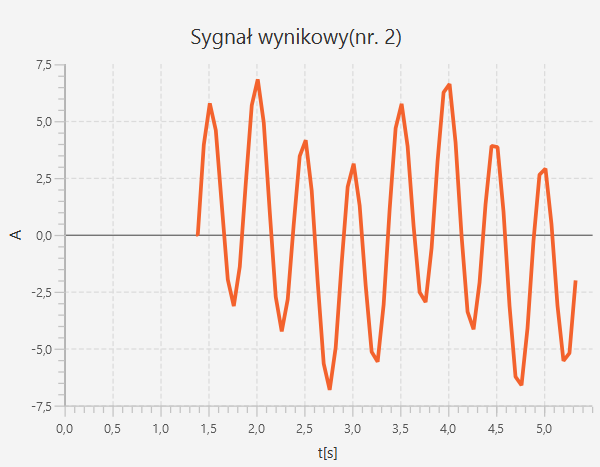
\includegraphics[width=\linewidth]{S1.png}
	\caption{Wykres sygnału S1}
	\label{S1_sygnal}
\end{figure}

% zeby wygenerować podałem dla sinusoidalnych wartosci:
% Pierwszy: A:2, ts: 0, czas trwania:4, T:2
% Drugi: A:1, ts:0, czas trwania:4, T:1
% i potem klkinałem "Dodaj do wygenrowanego; wtedy dodaje do shardkodowanego sygnału
\begin{figure}[H]
	\centering
	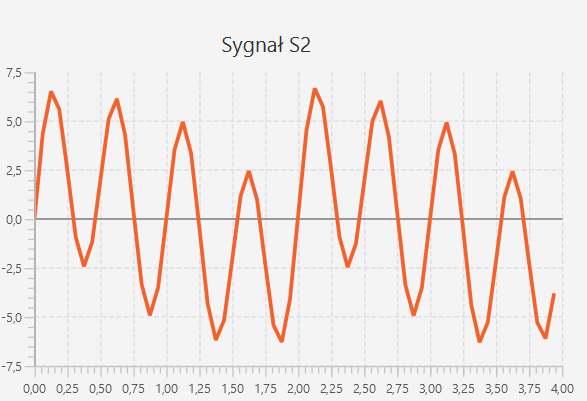
\includegraphics[width=\linewidth]{S2.png}
	\caption{Wykres sygnału S2}
	\label{S2_sygnal}
\end{figure}

% zeby wygenerować podałem dla sinusoidalnych wartosci:
% Pierwszy: A:5, ts: 0, czas trwania:4, T:2
% Drugi: A:1, ts:0, czas trwania:4, T:0.25

\begin{figure}[H]
	\centering
	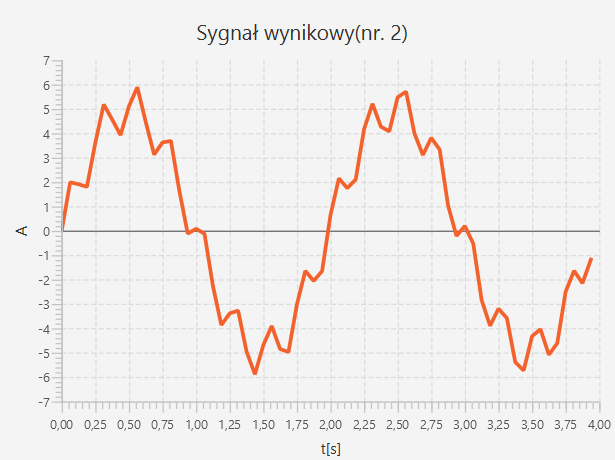
\includegraphics[width=\linewidth]{S3.png}
	\caption{Wykres sygnału S3}
	\label{S3_sygnal}
\end{figure}

\subsection{Dyskretna Transformacja Fouriera oraz Szybka Transformacja Fouriera}
Kolejnym etapem było wygenerowanie transformat dla powyżej przedstawionych sygnałów wykorzystując do tego algorytmy DFT oraz FFT. Podczas działania algorytmów mierzony był czas ich wykonania. Wyniki przedstawiamy poniżej. Wykresy są przedstawione zgodnie z instrukcją w dwóch trybach. W pierwszym z nich (W1) górny wykres prezentuje część rzeczywistą amplitudy w funkcji częstotliwości, a wykres dolny część urojoną, a w drugim (W2) górny wykres prezentuje moduł liczby zespolonej, a dolny argument liczby w funkcji częstotliwości.

\subsubsection{Dyskretna Transformacja Fouriera}
Sygnały będące wynikiem Dyskretnej Transformacji Fouriera przeprowadzonej dla sygnału S1 znajdującego się na rysunku \ref{S1_sygnal} prezentują się następująco:
\begin{figure}[H]
	\centering
	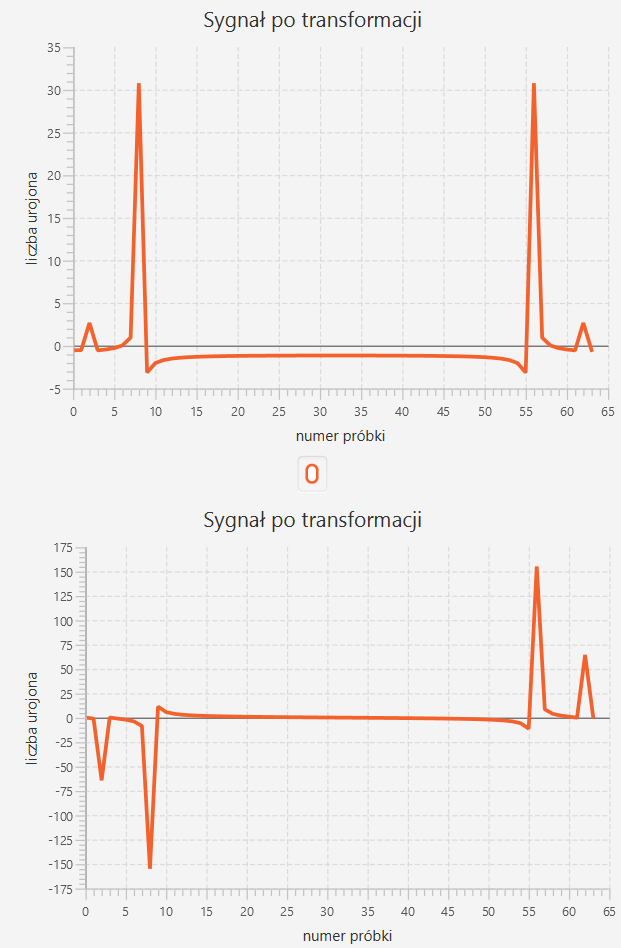
\includegraphics[width=\linewidth]{S1_DFT_W1.png}
	\caption{wykresy typu W1 dla DFT na sygnale S1}
	\label{S1_DFT_W1}
\end{figure}

\begin{figure}[H]
	\centering
	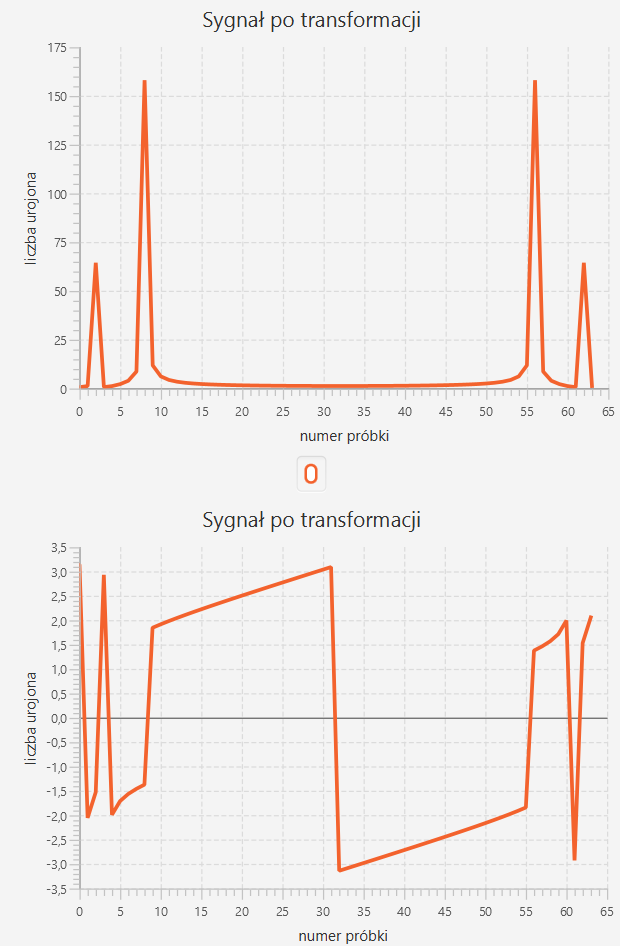
\includegraphics[width=\linewidth]{S1_DFT_W2.png}
	\caption{wykresy typu W2 dla DFT na sygnale S1}
	\label{S1_DFT_W2}
\end{figure}

Sygnały będące wynikiem Dyskretnej Transformacji Fouriera przeprowadzonej dla sygnału S2 znajdującego się na rysunku \ref{S2_sygnal} prezentują się następująco:
\begin{figure}[H]
	\centering
	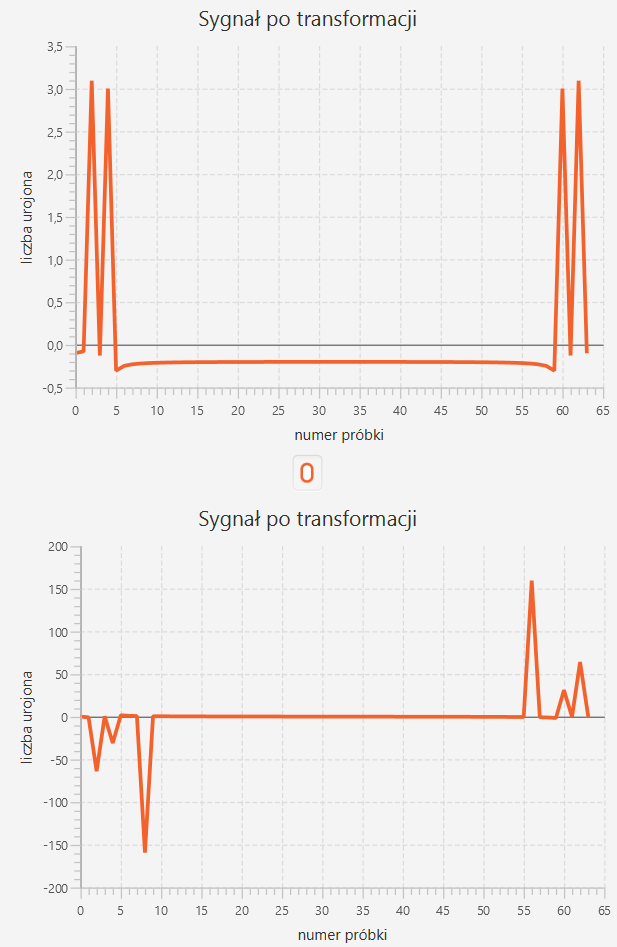
\includegraphics[width=\linewidth]{S2_DFT_W1.png}
	\caption{wykresy typu W1 dla DFT na sygnale S2}
	\label{S2_DFT_W1}
\end{figure}

\begin{figure}[H]
	\centering
	\includegraphics[width=\linewidth]{S2_DFT_W2.png}
	\caption{wykresy typu W2 dla DFT na sygnale S2}
	\label{S2_DFT_W2}
\end{figure}

Sygnały będące wynikiem Dyskretnej Transformacji Fouriera przeprowadzonej dla sygnału S3 znajdującego się na rysunku \ref{S3_sygnal} prezentują się następująco:
\begin{figure}[H]
	\centering
	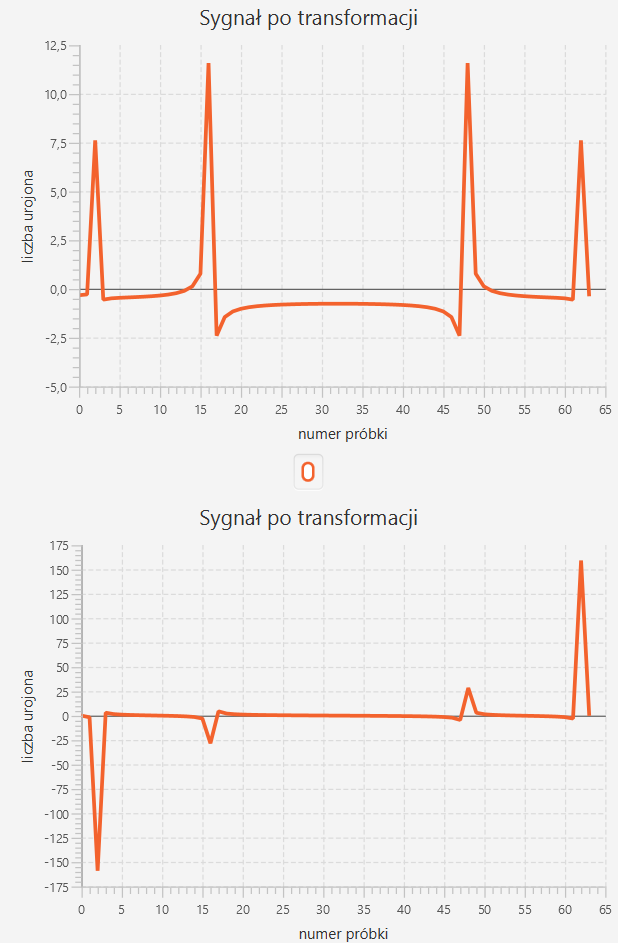
\includegraphics[width=\linewidth]{S3_DFT_W1.png}
	\caption{wykresy typu W1 dla DFT na sygnale S3}
	\label{S3_DFT_W1}
\end{figure}

\begin{figure}[H]
	\centering
	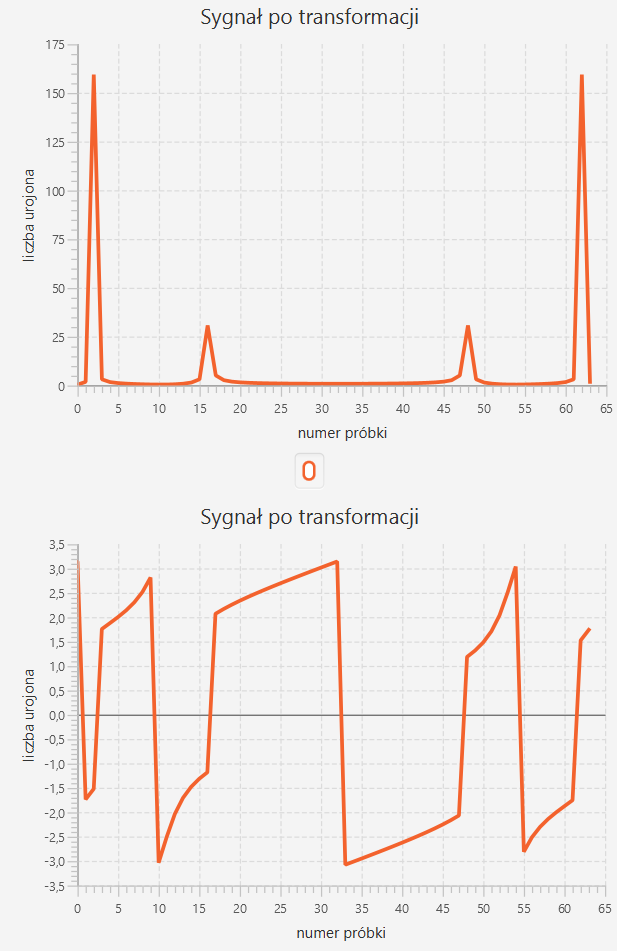
\includegraphics[width=\linewidth]{S3_DFT_W2.png}
	\caption{wykresy typu W2 dla DFT na sygnale S3}
	\label{S3_DFT_W2}
\end{figure}

\subsubsection{Szybka Transformacja Fouriera}
Sygnały będące wynikiem Szybkiej Transformacji Fouriera przeprowadzonej dla sygnału S1 znajdującego się na rysunku \ref{S1_sygnal} prezentują się następująco:
\begin{figure}[H]
	\centering
	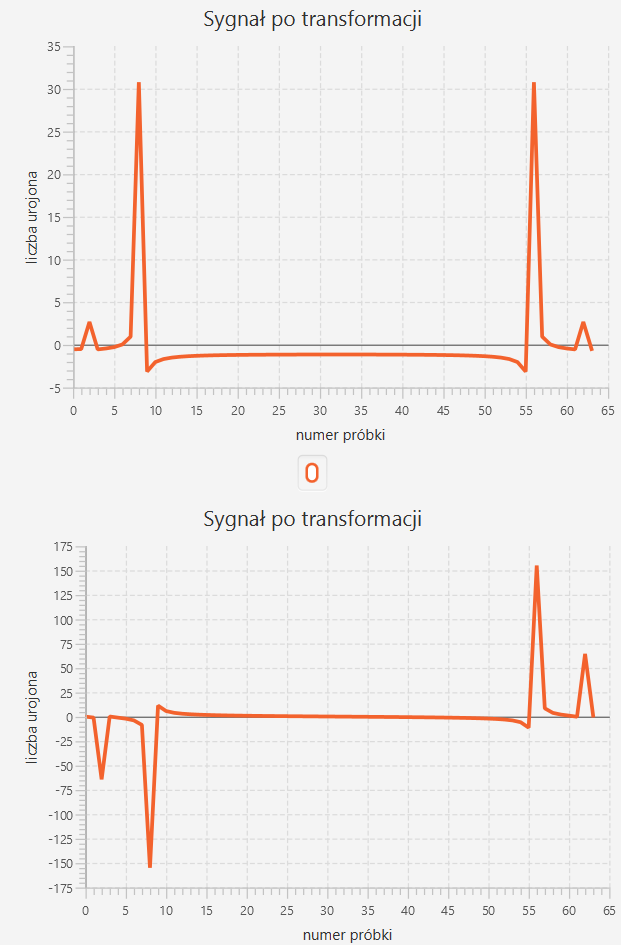
\includegraphics[width=\linewidth]{S1_FFT_W1.png}
	\caption{wykresy typu W1 dla FFT na sygnale S1}
	\label{S1_FFT_W1}
\end{figure}

\begin{figure}[H]
	\centering
	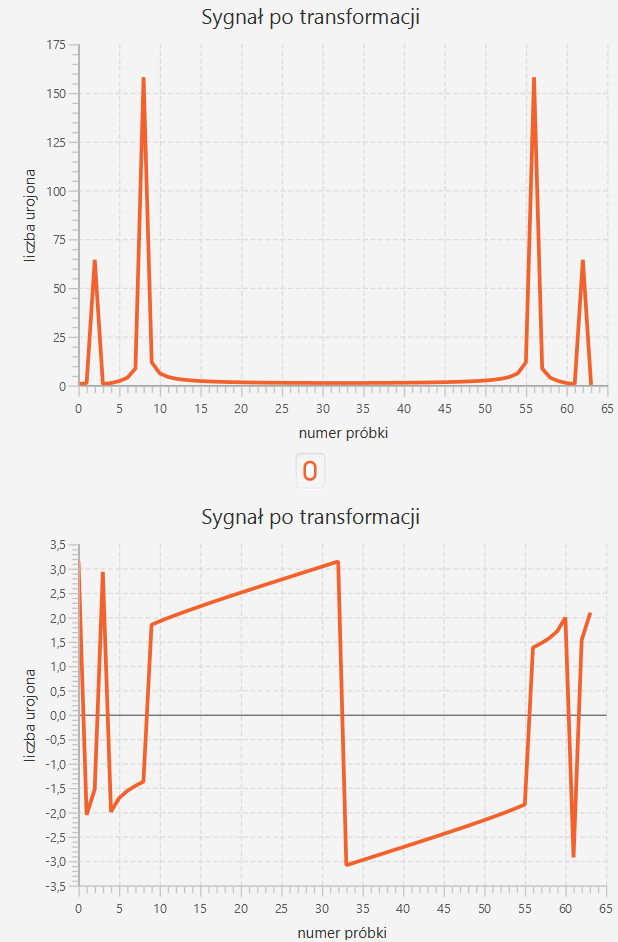
\includegraphics[width=\linewidth]{S1_FFT_W2.png}
	\caption{wykresy typu W2 dla FFT na sygnale S1}
	\label{S1_FFT_W2}
\end{figure}

Sygnały będące wynikiem Szybkiej Transformacji Fouriera przeprowadzonej dla sygnału S2 znajdującego się na rysunku \ref{S2_sygnal} prezentują się następująco:
\begin{figure}[H]
	\centering
	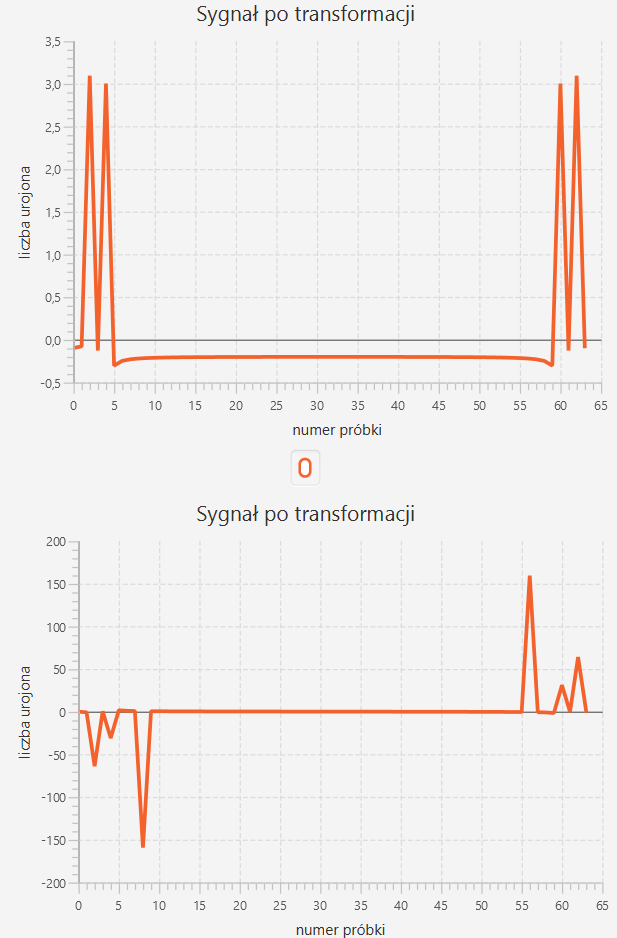
\includegraphics[width=\linewidth]{S2_FFT_W1.png}
	\caption{wykresy typu W1 dla FFT na sygnale S2}
	\label{S2_FFT_W1}
\end{figure}

\begin{figure}[H]
	\centering
	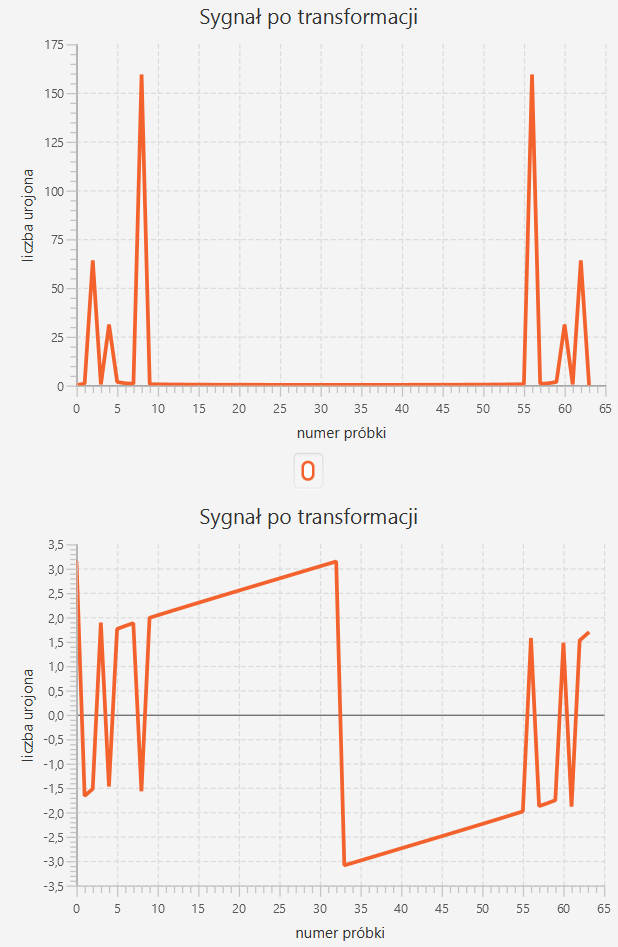
\includegraphics[width=\linewidth]{S2_FFT_W2.png}
	\caption{wykresy typu W2 dla FFT na sygnale S2}
	\label{S2_FFT_W2}
\end{figure}

Sygnały będące wynikiem Szybkiej Transformacji Fouriera przeprowadzonej dla sygnału S3 znajdującego się na rysunku \ref{S3_sygnal} prezentują się następująco:
\begin{figure}[H]
	\centering
	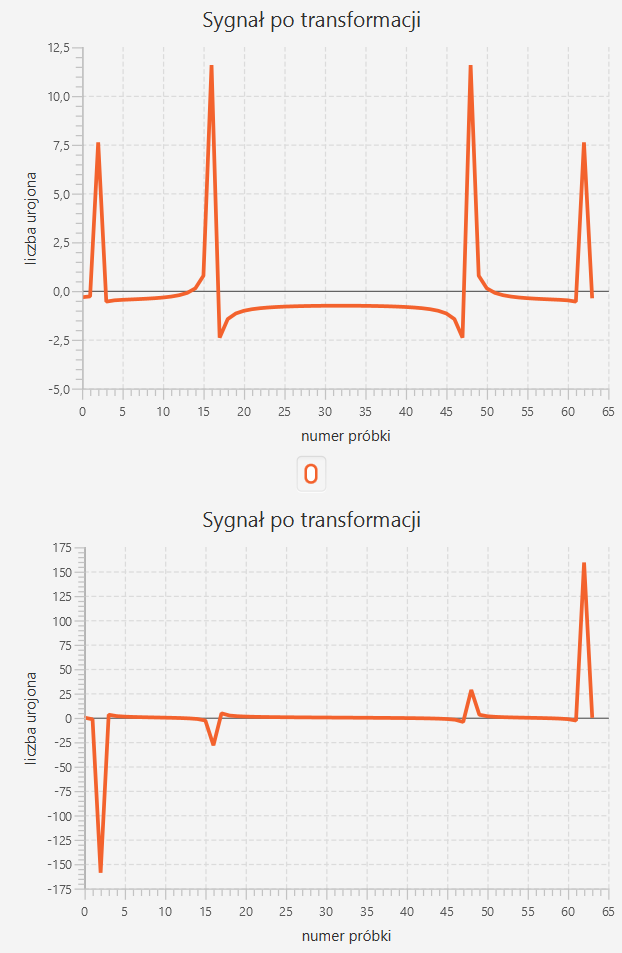
\includegraphics[width=\linewidth]{S3_FFT_W1.png}
	\caption{wykresy typu W1 dla FFT na sygnale S3}
	\label{S3_FFT_W1}
\end{figure}

\begin{figure}[H]
	\centering
	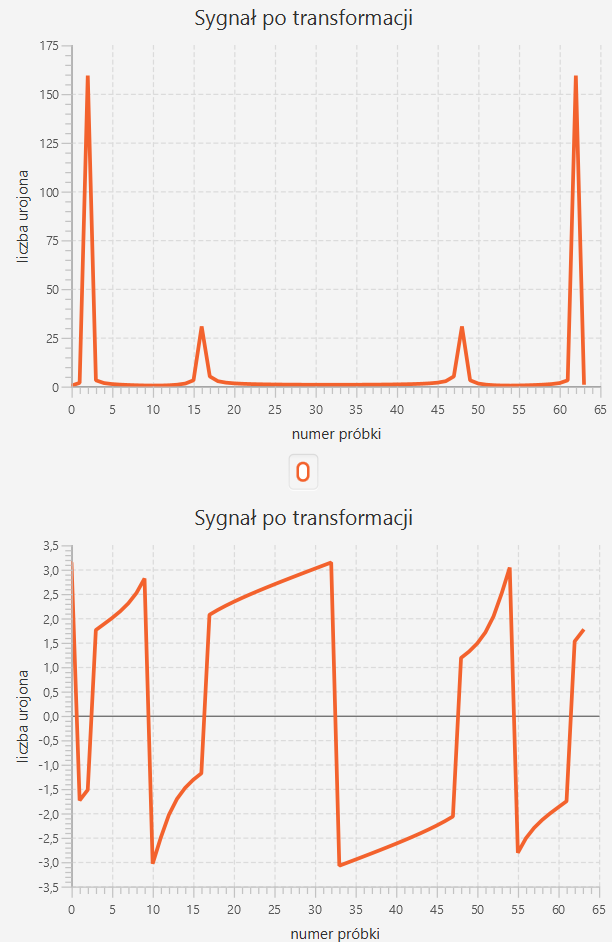
\includegraphics[width=\linewidth]{S3_FFT_W2.png}
	\caption{wykresy typu W2 dla FFT na sygnale S3}
	\label{S3_FFT_W2}
\end{figure}

\subsubsection{Porównanie czasów wykonania algorytmów DFT i FFT}
W ramach programu zaimplementowaliśmy także liczenie czasów wykonania poszczególnych transformacji. Zestawiając czasy wykonania dla Dyskretnej Transformacji Fouriera i Szybkiej Transformacji Fouriera otrzymamy następującą tabelę:

\begin{table}[H]
\centering
\begin{tabular}{|l|l|l|}
\hline
   & DFT     & FFT     \\ \hline
S1 & 5,24 ms & 0,42 ms \\ \hline
S2 & 2,17 ms & 0,47 ms \\ \hline
S3 & 2,55 ms & 0,41 ms \\ \hline
\end{tabular}
\end{table}
%%%%%%%%%%%%%%%%%%%%%%%%%%%%%%%%%%%%%%%%%%%%%%%%%%%%%%%%%%%%%%%%%%%%%%%%%%%%%%%%%%%%%%%%%%%%%%%%%%%%%%%%%%%%%%%%%

%%%%%%%%%%%%%%%%%%%%%%%%%%%%%%%%%%%%%%%%%%%%%%%%%%%%%%%%%%%%%%%%%%%%%%%%%%%%%%%%%%%%%%%%%%%%%%%%%%%%%%%%%%%%%%%%%
\section{Wnioski}
\indent
\indent Program został zaimplementowany prawidłowo i spełnia swoje funkcje jakimi było wygenerowanie transformat DFT, FFT i falkowa. Umożliwione zostało także wyświetlanie wyników w odpowiednim formacie (dwa tryby wyświetlania: (W1), w którym górny wykres prezentuje część rzeczywistą amplitudy w funkcji częstotliwości, a wykres dolny część urojoną i (W2), w którym górny wykres prezentuje moduł liczby zespolonej, a dolny argument liczby w funkcji częstotliwości.)\\

\indent Analizując wykresy dla Dyskretnej i dla Szybkiej Transformacji Fouriera możemy zauważyć, że wykresy transformat dla tych samych sygnałów wyglądają tak samo zarówno dla DFT, jak i FFT. Uważamy, że jest to jak najbardziej pożądane zachowanie programu. Patrząc na czasy wykonania obu algorytmów Szybka transformacja Fouriera jest w przypadku sygnału S2 ponad 4 razy szybsza, a w przypadku S1 nawet ponad 10 razy. Pokazuje to dlaczego w systemach informatycznych i telekomunikacyjnych wykorzystywana jest właśnie Szybka Transformacja Fouriera - ten sam wynik możemy otrzymać w zdecydowanie krótszym czasie.

%%%%%%%%%%%%%%%%%%%%%%%%%%%%%%%%%%%%%%%%%%%%%%%%%%%%%%%%%%%%%%%%%%%%%%%%%%%%%%%%%%%%%%%%%%%%%%%%%%%%%%%%%%%%%%%%%
% BIBLIOGRAFIA
%%%%%%%%%%%%%%%%%%%%%%%%%%%%%%%%%%%%%%%%%%%%%%%%%%%%%%%%%%%%%%%%%%%%%%%%%%%%%%%%%%%%%%%%%%%%%%%%%%%%%%%%%%%%%%%%%
\begin{thebibliography}{}
\bibitem{instrukcja} Instrukcja do zadania 4 na stronie przedmiotu. [przeglądany 26.05.2021], Dostępny w: https://ftims.edu.p.lodz.pl/pluginfile.php/14303/mod\_resource/content/0/zadanie4.pdf


\end{thebibliography}



\end{document}
